\documentclass[twoside]{article}
\usepackage{array}
\newcolumntype{L}{>{\arraybackslash}m{10cm}}
\usepackage{graphicx}
\usepackage{algorithm}% http://ctan.org/pkg/algorithm
\usepackage{algpseudocode}% http://ctan.org/pkg/algorithmicx
\usepackage{blindtext} % Package to generate dummy text throughout this template 
\usepackage{physics}
\usepackage[sc]{mathpazo} % Use the Palatino font
\usepackage[T1]{fontenc} % Use 8-bit encoding that has 256 glyphs
\linespread{1.05} % Line spacing - Palatino needs more space between lines
\usepackage{microtype} % Slightly tweak font spacing for aesthetics
\algnewcommand{\LeftComment}[1]{\Statex \(\triangleright\) #1}
\usepackage[english]{babel} % Language hyphenation and typographical rules
\usepackage{color,soul}

\usepackage[hmarginratio=1:1,top=32mm,columnsep=20pt]{geometry} % Document margins
\usepackage[hang, small,labelfont=bf,up,textfont=it,up]{caption} % Custom captions under/above floats in tables or figures
\usepackage{booktabs} % Horizontal rules in tables

\usepackage{lettrine} % The lettrine is the first enlarged letter at the beginning of the text

\usepackage{enumitem} % Customized lists
\setlist[itemize]{noitemsep} % Make itemize lists more compact

\usepackage{abstract} % Allows abstract customization
\renewcommand{\abstractnamefont}{\normalfont\bfseries} % Set the "Abstract" text to bold
\renewcommand{\abstracttextfont}{\normalfont\small\itshape} % Set the abstract itself to small italic text

\usepackage{titlesec} % Allows customization of titles
%\renewcommand\thesection{\Roman{section}} % Roman numerals for the sections
%\renewcommand\thesubsection{\roman{subsection}} % roman numerals for subsections
\titleformat{\section}[block]{\large\scshape\centering}{\thesection.}{1em}{} % Change the look of the section titles
\titleformat{\subsection}[block]{\large}{\thesubsection.}{1em}{} % Change the look of the section titles

\usepackage{fancyhdr} % Headers and footers
\pagestyle{fancy} % All pages have headers and footers
\fancyhead{} % Blank out the default header
\fancyfoot{} % Blank out the default footer
\fancyhead[C]{Word Recommendation For Crosswords Using Distributed Words Embedding $\bullet$ Nov 2019} % Custom header text
\fancyfoot[RO,LE]{\thepage} % Custom footer text
\setul{0.5ex}{0.3ex}
\setulcolor{red}

\usepackage{titling} % Customizing the title section

\usepackage{hyperref} % For hyperlinks in the PDF
\usepackage{amsmath}
\DeclareMathOperator*{\argmax}{arg\,max}
\DeclareMathOperator*{\argmin}{arg\,min}

%----------------------------------------------------------------------------------------
%	TITLE SECTION
%----------------------------------------------------------------------------------------

\setlength{\droptitle}{-4\baselineskip} % Move the title up

\pretitle{\begin{center}\Huge\bfseries} % Article title formatting
\posttitle{\end{center}} % Article title closing formatting
\title{Word Recommendation For Crosswords Using Distributed Words Embedding } % Article title
\author{%
\textsc{Charu Agarwal} \\[1ex] % Your name
\normalsize Indian Insitute of Technology, Dharwad \\ % Your institution
\normalsize \href{mailto:160010038@iitdh.ac.in}{160010038@iitdh.ac.in} % Your email address
}
\date{\today} % Leave empty to omit a date
\renewcommand{\maketitlehookd}{%
\begin{abstract}
\begin{center}
\noindent In this paper, we consider the problem of creating thematic crosswords from seed words. Typically, human constructors select words and clues based on some theme around which the grid can be created. Modern constructors frequently use software to speed the task of filling the rest of the grid. Although several programs are available for this task, they do not create themes and do not create a fill that is dense and thematic. We propose novel neural language-based algorithms specifically tailored to suggest effective word recommendations for crosswords. We prototype and test these algorithms against realistic inputs. We find that our technique is feasible, often suggesting good words. We also shed some light on algorithmic options.
\end{center}
\end{abstract}
}

%----------------------------------------------------------------------------------------

\begin{document}

% Print the title
\maketitle

%----------------------------------------------------------------------------------------
%	ARTICLE CONTENTS
%----------------------------------------------------------------------------------------

\section{Introduction}
\label{sec:sec1}
\lettrine[nindent=0em,lines=3]{C} rosswords are word puzzles that usually take the form of a square or a rectangular grid of white- and black-shaded squares. The game's goal is to fill the white squares with letters, forming words or phrases, by solving clues, which lead to the answers. Usually, the answer words and phrases are placed in the grid from left to right and from top to bottom. The black squares are used to separate words or phrases.

Ever since their introduction in 1913 by Arthur Wayne, crossword puzzles are used every day by millions of people not only for entertainment but also have applications in educational and rehabilitation contexts. As actress Betty White states: ``I don't have any trouble memorizing lines because of the crossword puzzles I do every day to keep my mind a little limber''. Crosswords are absorbing and fascinating, giving a mild amount of mental stimulation and recreation at the same time. They form an essential part of newspapers and magazines, and more recently are being used by organizations and schools as a teaching tool \cite{cite1}, for example, it has been used to study sociological concepts \cite{cite2} and medical concepts \cite{cite3}.

Crossword construction is a difficult and complex art and is mainly done by experts. There are two main parts to the crossword construction problem: (1) selecting a "good" set of words to be fitted in a crossword and, (2) given a set of words, fitting the words in a grid while respecting the constraints of the crossword. While much work has been done for (2), by posing the crossword construction problem as a constraint satisfaction problem \cite{cite4} or a heuristic-based search problem \cite{cite5}, the problem of (1) is still largely unsolved.

Crossword puzzles often have a theme, that is, the set of words to be filled in the crossword come from a theme. Category theme puzzles have theme elements as members of the same set, eg. parts of a tree. Anniversary or tribute theme puzzles commemorate a specific person, place, or event eg. on October 7, 2011 The New York Times crossword commemorated the life of Apple CEO Steve Jobs who had died on October 5 which included words such as 'STEVE JOBS', 'IPOD', 'APPLE', 'MACINTOSH', among others. Synonym theme puzzles have the theme entries all contain synonyms e.g., a Los Angeles Times puzzle featuring a set of theme entries that contain the words RAVEN, JET, EBONY, and SABLE, all synonyms for "black". Typical crossword puzzles contain 4-5 theme entries and the rest of the entries are filled using a software, with particularly bad or obscure entries edited out by human experts.

The generation of thematic puzzles on specific subjects typically requires a great deal of human expert work. Software systems such as Crossword Compiler, CrossFire, Dr. Fill \cite{cite6} and PuzzleMe have been created to speed up the process. However, none of these generate puzzles based on cohesive themes automatically. We exemplify this point with an example in figure \ref{fig:figbox} where we compare the results of our algorithm with a standard gridfilling software .

\subsection{Our key contributions}
\begin{itemize}
  \item We propose new techniques of suggesting themed words for a crossword given seed words and clues. The main idea is that we leverage word semantics as captured by high-dimensional distributed word embeddings. 
  \item We have created a working prototype system for recommmending words for Amuse Labs, a leading provider of crosswords. The effort included developing a product-level word suggestion algorithm based on the given word and clues, capable of giving near real-time suggestions to the users.
  \item We have evaluated the algorithm and the system by considering realistic examples.
\end{itemize} 

\subsection{Organization of the report}
The rest of the report is organized as follows. Section \ref{sec:sec2} gives a brief overview of related work and word vector representations. Section \ref{sec:sec3} describes our methodology to suggest words for the crossword. Section \ref{sec:sec4} presents a method to generate distributed word embeddings from domain-specific corpora. Section \ref{sec:sec5} describes an attempt to derive relations between clues and answers. Section \ref{sec:sec6} explains the system developed. Finally, section \ref{sec:sec7} briefly discusses the results and section \ref{sec:sec8} concludes.

\section{Related Work}
\label{sec:sec2}
In WebCrow-generation\cite{cite7}, topic-specific crosswords\footnote{ A topic-specific crossword is a crossword having most of the definition/answer pairs belonging to a given topic T.}  are automatically generated where a user specifies a set of topics of expertise, and the automatic system generates a crossword that is targeted to his/her skills. While the results are good, this will not work in the case where the topic is not explicitly specified. In the most natural case, the designer would like to extend the words list by adding more related words to the crossword. For example, if a crossword designer suggests the words ‘XMAS TREE’, ‘SANTA’ and ‘REINDEER’, then it can be understood that the expert wants to design a Christmas themed puzzle.

The lexical relations encoded in WordNet,  a human-curated lexical database,  have been used in \cite{cite8} to enhance the aesthetics of the resulting crossword, to construct crosswords with a thematic focus. However, this approach has several limitations as WordNet does not include much domain-specific terminology and does not uncover certain types of semantic relations.

\begin{figure}[H]
\fbox{\begin{minipage}{\textwidth}
To illustrate the need for themed word suggestions, we ran our algorithm on a sample crossword puzzle with the theme Gandhi. Figure \ref{fig:fig1} shows the crossword, along with some of the words suggested, highlighted in red. We can observe that a lot of closely related words to the theme have been suggested. For example, ‘Sabarmati Ashram’ is the famous residence of Gandhi. ‘Harijans’ was a term popularized by Gandhi to give respect to the communities that were traditionally labeled as untouchables. ‘Hind Swaraj’ is the title of a book authored by Gandhi. ‘Bapu’ is another name of Gandhi. Just as a comparison, we used a popular crossword construction tool Sparkling Fill\footnote{https://sparklingfill.com/} to suggest words for the same set of input words. While from the layout point of view, Sparkling Fill definitely improves the fill of the grid, it is not clear how words such as ‘AAA’, ‘LII’, ‘WET’, ‘TRA’, ‘EEK’ and, ‘GREET’ classify as a good fill. Of course, if we have a clever clue designer, it might be possible to overcome this difficulty, but it is difficult to use such words in general without reducing the quality of the crossword.
\begin{center}
    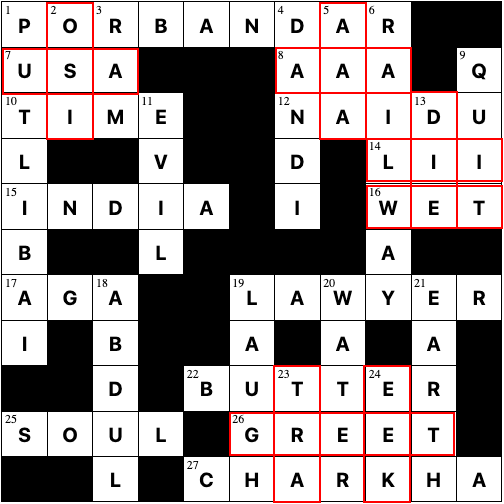
\includegraphics[height=175pt]{images/crossword_gandhi_fill.png}
    \hspace{1cm}
    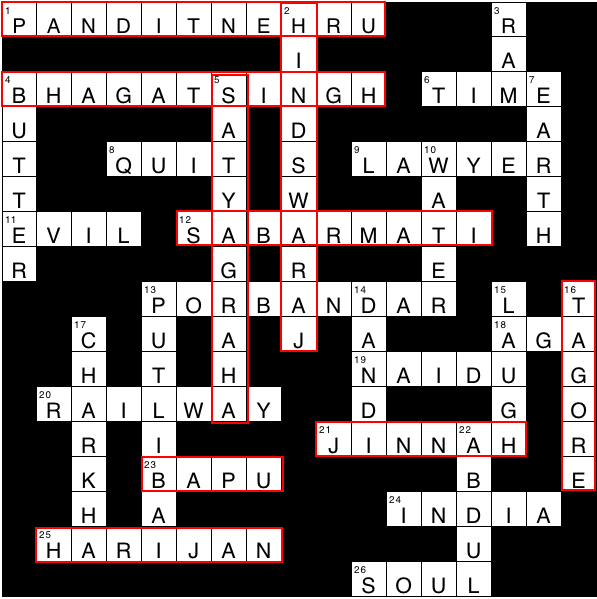
\includegraphics[height=175pt]{images/crossword_gandhi.png}
   \captionof{figure}{Crossword based on the theme ‘Mahatma Gandhi’. In the left image, the words highlighted in red have been suggested using the Sparkling Fill tool. In the right image, words highlighted in red have been suggested using the distributed word embeddings of the answers and the clues.}
   \label{fig:fig1}
   \end{center}
\end{minipage}}
\caption{Example result from our word recommendation algorithm, compared to a standard grid filling software. The puzzle used in this example was published by the Hindu on October 2, 2019 to commemorate Mahatma Gandhi's 150th birthday.}
\label{fig:figbox}
\end{figure}

Our algorithm is based on the recent work in learning word vector representations using neural networks \cite{cite9} \cite{cite10} \cite{cite11} \cite{cite12} \cite{cite13}. The idea is that a word is represented by context in use. For example, consider the following two sentences: (1) I eat an \textit{apple} everyday. (2) I eat an \textit{orange} everyday. Since apple and orange are used in similar contexts, it might suggest that there is some similarity relation between these two words. In this formulation, each word is represented by a vector that is concatenated or averaged with other word vectors in a context, and the resulting vector is used to predict other words in the context.

The outcome is that after the model is trained, the word vectors are mapped into a vector space such that semantically-similar words have similar word representations (e.g. “happy” is close to “pleased”). \cite{cite9} used a feedforward neural network with a linear projection layer and a non-linear hidden layer to jointly learn the word vector representations and a statistical language model. \cite{cite10} and \cite{cite11}  leveraged distributed word vectors to show that neural network based models match or outperform feature-engineered systems for standard Natural Language Processing (NLP) tasks that include part-of-speech tagging, chunking, named entity recognition, and semantic role labeling. \cite{cite14} introduced a technique to learn better word embeddings by incorporating both local and global document context, and account for homonymy and polysemy by learning multiple embeddings per word. \cite{cite15} \cite{cite16} \cite{cite17} introduced Word2Vec and the Skip-gram model, a very simple method for learning word vectors from large amounts of unstructured text data. The model avoids non-linear transformations and therefore makes training extremely efficient. This enables learning of high dimensional word vectors from huge datasets with billions of words, and millions of words in the vocabulary. \\High-dimensional word vectors can capture subtle semantic relationships between words. For example, word vectors can be used to answer analogy questions using simple vector algebra: $v_{king} - v_{man} + v_{woman} = v_{queen}$, where $v_x$ denotes the vector for the word $x$. \cite{cite18} later introduced GloVe, Global Vectors for Word Representation, which combines word-word global co-occurrence statistics from a corpus, and context based learning similar to Word2Vec to deliver an improved word vector representation.
Recently, Doc2Vec \cite{cite24} was proposed as an extension to Word2Vec to learn document-level embeddings for sentences and paragraphs. A model that learns dense word vectors jointly with Dirichlet-distributed latent document-level mixtures of topic vectors was introduced in \cite{cite25}.
\\ Word vectors are an attractive building block and are being used as input for many neural net based natural language tasks such as sentiment analysis \cite{cite19} \cite{cite20}, question and answer systems, \cite{cite21} \cite{cite22}, and others. More recently, the technique has been applied to recommenders and advertising \cite{cite23}. These powerful, efficient models have shown very promising results in capturing both syntactic and semantic relationships between words in largescale text corpora, obtaining state-of-the-art results on a plethora of NLP tasks.

\section{Methodology}
\label{sec:sec3}
In this section, we describe our algorithm for generating word suggestions from a given set of clues and answers. Our approach consists of three steps. First, we extract the nouns from the clues which involves sentence segmentation, tokenization and parts of speech tagging. Next, using the word embedding, we find the closest words for each clue-answer set. The clues help in adding context to the answer. Finally, we find the top-N most similar words and rank them based on importance. Algorithm \ref{algo:algo1} describes all the steps. We will use the example of the Gandhi puzzle shown in Figure \ref{fig:figbox} to explain all the steps of the algorithm, while providing empirical results\footnote{While we suggest different strategies for each step, our goal is to not classify which one is better. The results are given just to get a sense of the different strategies.}. Table \ref{tab:table1} shows the clues and the answers for the puzzle. Figure \ref{fig:algo_schematic} shows a schematic diagram of the algorithm. 

\begin{figure*}
  \centering
  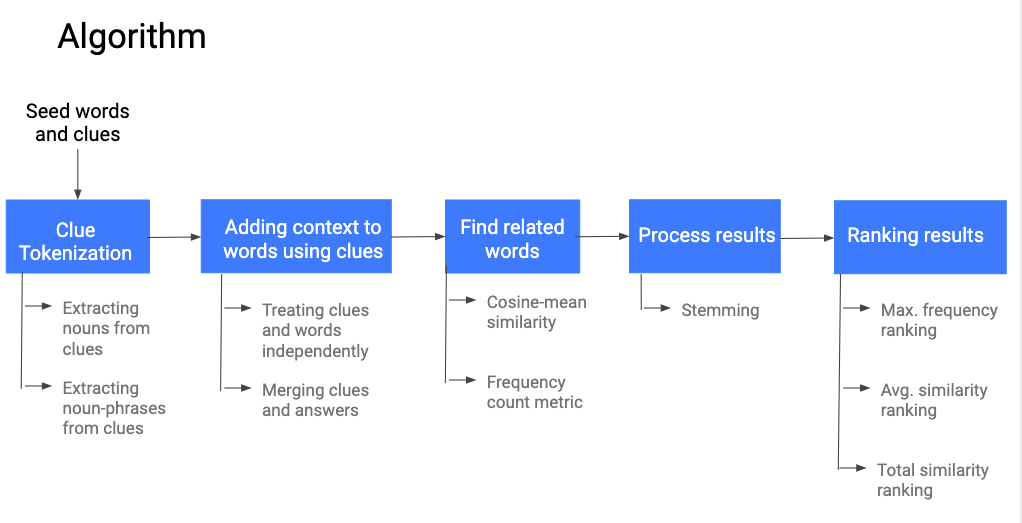
\includegraphics[height=200pt]{images/algo_schematic.png}
  \caption{Schematic Diagram of the algorithm for suggesting words for crossword.}
  \label{fig:algo_schematic}
\end{figure*}

\begin{algorithm}
  \caption{Algorithm to suggest themed-words for a crossword.}\label{algo:algo1}
  \begin{algorithmic}[1]
    \Procedure{suggest\_words}{model, words\_list, clues\_list}\Comment{Returns word suggestions for a crossword grid.}


      \State $clue\_nouns \gets extract\_clue\_nouns(clues\_list)$ \Comment{Tokenize clues. Ref. section \ref{sec:sec3.3}.}\\

       \LeftComment{Combine clues and answers. Ref. section \ref{sec:sec3.4}.}
      \State $clue\_words\_combined \gets combine(words\_list, clues\_nouns)$\\
      \LeftComment{Filter words not in model vocabulary.} \\
      $filter\_words\_not\_in\_vocab(model, clue\_words\_combined)$ 
      \\
      \LeftComment{Find related words. Ref. section \ref{sec:sec3.2}.}
      \State $word\_suggestions \gets get\_related\_words(clue\_words\_combined)$ 
      \\
      \LeftComment{Process the results. Ref. section \ref{sec:sec3.5}.}
      \State $processed\_results \gets process\_results(word\_suggestions)$ \\
      \LeftComment{Rank the results. Ref. section \ref{sec:sec3.6}.}
      \State $ranked\_suggestions \gets rank\_words(processed\_results, words\_list, clues\_list, model)$ \\
      \State \textbf{return} $ranked\_suggestions$  
      \EndProcedure
  \end{algorithmic}
\end{algorithm}

\begin{table}[h!]
  \begin{center}
    \begin{tabular}{c L}
      \toprule
      \textbf{Answer} & \textbf{Clue}  \\ 
      \midrule
      Porbandar & Gandhi's birthplace\\
      Putli Bai & Gandhi's mother\\
      Ram & Hey $\rule{1cm}{0.15mm}$ : Gandhi's last words\\
      Time & Gandhi was $\rule{1cm}{0.15mm}$  Magazine's Man of the Year in 1930\\
      India & Young $\rule{1cm}{0.15mm}$ : A journal published by Gandhi\\
      Aga & Gandhi and Kasturba were jailed at $\rule{1cm}{0.15mm}$  Khan's palace\\
      Abdul & $\rule{1cm}{0.15mm}$  Khan Gaffar Khan was also known as Frontier Gandhi\\
      Soul & Mahatma means Great $\rule{1cm}{0.15mm}$ \\
      Charkha & The spinning wheel made iconic by Gandhi\\
      butter & The villagers want bread not $\rule{1cm}{0.15mm}$ : quote by Gandhi\\
      lawyer & Gandhi's profession in South Africa\\
      Naidu & Sarojni $\rule{1cm}{0.15mm}$  became president of the Indian National Congress after Gandhi\\
      Railway & Gandhi was thrown out of the train at Pietermaritzburg $\rule{1cm}{0.15mm}$  Station\\
      Quit & Gandhi started the $\rule{1cm}{0.15mm}$  India Movement in 1942\\
      laugh & First they ignore you, then they $\rule{1cm}{0.15mm}$  at you, then they fight you, then you win: quote by Gandhi\\
      water & We may not be God, but we are of God, even as a little $\rule{1cm}{0.15mm}$  drop is of the ocean: quote by Gandhi \\
      earth & $\rule{1cm}{0.15mm}$ provides enough to satify every man's needs, but not every man's greed: quote by Gandhi\\
      evil & Good and $\rule{1cm}{0.15mm}$ are found together: quote by Gandhi\\
      Dandi & Gandhi led the Salt March to this beach\\
      \bottomrule
    \end{tabular}
    \caption{Running example seed input for puzzle published by the Hindu in commemoration of Mahatma Gandhi's 150th birthday.}
    \label{tab:table1}
  \end{center}
\end{table}

\subsection{Word Embeddings}
\label{sec:sec3.1}
For the word embeddings, we used a model published by Google, which was trained on 100 billion words from a Google News dataset\footnote{https://code.google.com/archive/p/word2vec/}. The model contains 300-dimensional vectors for 3 million words and phrases. The reason for choosing this dataset was that modern crosswords allow many non-dictionary words and phrases too. For example, some words only became popular (in terms of the crossword) in recent years: 'BAE' and 'LGBT' appeared four and five time respectively in the year 2017 in the New York Times crosswords \cite{cite26}. News is the best source of upcoming trends and modern vocabulary.

\subsection{Finding related words}
\label{sec:sec3.2}
We first used only the answers to find word recommendations. Two metrics were used:
\begin{enumerate}
  \item Cosine-mean similarity: This method computes cosine similarity between a simple mean of the projection weight vectors of the given words and returns the top-N most similar vecs from the training set.
  \begin{equation}
  similarity = cos\theta = \frac{X.Y}{\norm{X}.\norm{Y}}
  \end{equation}
  \item Frequency count: This method finds the words which occur most number of times within top-N cosine distance of each input word.
\end{enumerate}
Table \ref{tab:table2} shows the results of applying both the metrics on the Gandhi puzzle. 'Karmabhoomi' was a novel inspired by Gandhi's satyagraha movement. The rest of the words from metric 1 are not very related to Gandhi, but more to politicians and the last word 'By Riyanki Das' is the name of a reporter, taken from an article. In contrast, 'Gujarat' was the birthplace of Gandhi, 'Bhavnagar' is the place where Gandhi received their education, and there is a Mahatma Gandhi (M.G.) road in 'Junagadh'. Frequency count metric performs better for this puzzle\footnote{All evaluations have been done qualitatively, may vary from person to person.}. We ran the two metrics on diverse themed puzzles and found that, in most cases, the frequency count metric gives much better results.

\begin{table}[h!]
  \begin{center}
    \begin{tabular}{c c}
      \toprule
      \textbf{Cosine-mean similarity metric} & \textbf{Frequency count metric}  \\ 
      \midrule
      \ul{karma bhoomi} & \ul{Gujarat} \\
      Birwa & \ul{Porbander}\\
      Lalooji & \ul{Bhavnagar}\\
      Shastriji & Valsad\\
      By Riyanki Das & \ul{Junagadh}\\
      Photo C. Ratheesh & \ul{Navsari} \\
      Dutt saab & Bharuch \\
      AP Photo Bikas & Ramanathapuram\\
      Subhendu & Amreli \\
      sanyasi & Bhatkal\\
      \bottomrule
    \end{tabular}
     \caption{Top 10 words suggested using the cosine-mean similarity metric and the frequency count metric for the Gandhi puzzle answers. The themed words correctly suggested are highlighted in red.}
    \label{tab:table2}
  \end{center}
\end{table}

\subsection{Using clues to disambiguate words}
\label{sec:sec3.3}
We exploit the fact that in our problem domain, we not only have words but also clues, which can help in disambiguating the words. For example, the word 'Donald' alone may be ambiguous, but '$\rule{1cm}{0.15mm}$ Trump' or '$\rule{1cm}{0.15mm}$ Duck' will certainly add context. Going by this intuition, we decided to use the clues as well. We used two methods to tokenize the clues using standard natural language processing libraries:
\begin{enumerate}
  \item Extracting nouns from clues
  \item Extracting noun-phrases from clues
\end{enumerate}
Table \ref{tab:table3} shows the results of tokenizing the Gandhi puzzle clues. We observe that extracting nouns works better, since some words are lost while extracting noun phrases. 
\begin{table}[h!]
  \begin{center}
    \begin{tabular}{c c}
      \toprule
      \textbf{Nouns extracted} & \textbf{Noun-phrases extracted}  \\ 
      \midrule
      $['Gandhi', 'birthplace']$ & $['Gandhi']$ \\
      $['Gandhi', 'mother']$ & $['Gandhi']$\\
      $['Hey', 'Gandhi', 'words']$ & $['Gandhi']$\\
      $['Gandhi', 'Magazine', 'Man', 'Year']$ & $['Gandhi', 'Magazine']$\\
      $['Young', 'journal', 'Gandhi']$ & $['Young']$\\
      \bottomrule
    \end{tabular}
    \caption{First 5 clues tokenized for the Gandhi puzzle.}
    \label{tab:table3}
  \end{center}
\end{table}
 
\subsubsection{Generating noun-phrases from clues and answers}
Since the standard libraries were not able to find good noun-phrases, we decided to find phrases of variable length by combining adjacent words in the clues and querying them in the Google News model. For the Gandhi puzzle, we found four noun-phrases from the clues and the answers: ['Aga\_Khan', 'Abdul\_Gaffar', 'Dandi\_March', 'South\_Africa']. While this technique helped in finding phrases, it did not show significant improvement in the results for our example. Nevertheless, this idea of combining words to form phrases will definitely make the input more meaningful. 

\subsection{Method of combining clue and answers}
\label{sec:sec3.4}
To use the clues and the answers together, we considered two heuristic methods:
\begin{enumerate}
\item Treating clue nouns and answers independently: In this approach, we simply added the clue nouns to the input list and used this words list to find similar words using the frequency count metric.
\item Merging the clues and the answers: In this approach, we first merge the clue nouns and the answer to generate k most-similar words. That is, for each clue $c_i$ and the corresponding word $w_i$, we compute the cosine similarity between a simple mean of the projection weight vectors of $c_i$  and $w_i$ to compute the top-k most similar words $mean_i$. Using this list of $mean_i's$, we find similar words using the frequency count metric. This seemed intuitive as we want to capture the relation between the clues and the corresponding answers.

\end{enumerate}
Table \ref{tab:table4} shows the results of applying both methods on the Gandhi puzzle. If we treat each word independently, the model is not able to differentiate Mahatama Gandhi from Rahul Gandhi (an Indian politician) as both have Gandhi surname, due to which names of other politicians such as Karunanidhi and Gadkari are suggested. However, if we do not break the link between the clue and the answers, the model has a better understanding that Gandhi refers to the great freedom fighter Mahatma Gandhi, and hence very related words such as Sabarmati Ashram (Gandhi's Residence), Satyagraha (movement started by Gandhi), Vinobha Bhave (spiritual successor of Mohandas Gandhi), are suggested. Merging clue and answers performs better for this puzzle.

\begin{table}[h!]
  \begin{center}
    \begin{tabular}{c c}
      \toprule
      \textbf{Without merging} & \textbf{With merging}  \\ 
      \midrule
      \ul{salt satyagraha} & \ul{Sabarmati Ashram} \\
      Karunanidhi & Shivaji Maharaj\\
      Gadkari & \ul{satyagraha}\\
      Joshi & \ul{Acharya Vinoba Bhave}\\
      \ul{Vinoba} & \ul{Swami Vivekananda} \\
      \ul{Bapu} & \ul{Bapu} \\
      \ul{Ambedkar} & \ul{Ambedkar} \\
      \ul{Pandit Nehru} & \ul{Hind Swaraj} \\
      \ul{Swami Vivekananda}& \ul{Pandit Nehru} \\
      \ul{Tagore} & \ul{Sree Narayana Guru} \\
      \bottomrule
    \end{tabular}
    \caption{Top 10 words suggested using the clues and the answers for the Gandhi puzzle. In the first column, the clue words and the answer words are treated independently, while in the second column, the clue words and the answer words are averaged by finding the closest word to each clue-answer pair, and then used to generate the result words. The themed words correctly suggested are highlighted in red.}
    \label{tab:table4}
  \end{center}
\end{table}

\subsection{Processing results}
\label{sec:sec3.5}
The model contains a lot of words which are almost same, for example, 'Gandhi', 'Gandhian', 'Gandhi ji', 'Mahatma Gandhiji',
'Mahatma', 'Mahatama Gandhi', 'Mohandas Gandhi', 'Mohandas Karamchand Gandhi'. Also, there are many misspellings of the same word in the model. For example, one of the closest words to 'Porbandar' is 'Porbander'. Since we do not want morphological variants of the same word suggested, we use a stemming algorithm which filters out words which have the same root/base as the input words, or the result words. The algorithm reduces the words “chocolates”, “chocolatey”, “choco” to the root word, “chocolate” and “retrieval”, “retrieved”, “retrieves” reduce to the stem “retrieve”. Also, we remove duplicate words which only differ in the case. This is needed as the Google News model is case-sensitive. This helps us to promote diversity in the recommendations. 
Table \ref{tab:table5} shows the results of applying the stemming algorithm on the results for the Gandhi puzzle. Clearly, more good words come to top by filtering words with the same root.
\begin{table}[h!]
  \begin{center}
    \begin{tabular}{c c}
      \toprule
      \textbf{Before filtering} & \textbf{After filtering}  \\ 
      \midrule
      Sabarmati Ashram & Sabarmati Ashram \\
      Shivaji Maharaj & Shivaji Maharaj\\
      Gandhi & satyagraha\\
      Gandhian & Acharya Vinoba Bhave\\
      Gandhi ji & Swami Vivekananda \\
      \bottomrule
    \end{tabular}
    \caption{Top 5 words suggested using the clues and the answers for the Gandhi puzzle before and after using a stemming algorithm to filter out words with the same root.}
    \label{tab:table5}
  \end{center}
\end{table}

\subsection{Ranking of result words.}
\label{sec:sec3.6}
The final most important step is to rank the result words based on their importance. For each result word, we consider the input words which have generated the word. We considered three metrics for ranking:
\begin{enumerate}
  \item Max frequency ranking: This metric ranks the words based on the number of input words which lie within $\delta$ distance of the result word.
  \item Average similarity ranking: This metric ranks the words based on the average similarity from the input words.
  \item Total similarity ranking: This metric ranks the words based on the sum of similarity from each word. This metric takes account of both frequency and the similarity of the word.
\end{enumerate}
Table \ref{tab:table6} shows the results of applying the different rankings to the result words. It is not clear which ranking is better than the others.

We wanted to observe the effect of input size on the accuracy of the results. Figure \ref{fig:fig3.6} shows the number of themed words correctly suggested out of top 10 words suggested by both methods described in \ref{sec:sec3.4} based on the input size. For small input sizes, the method of using the clues and answers independently works better. For larger inputs, it is better to merge the clue and the answers first. This may be due to increase in the number of noise words as the size of the input words increases. Merging the clue and the answers may help in reducing the noise. Figure \ref{fig:fig3.6.1} summarizes the techniques discussed in this section.

\begin{figure*}
  \centering
  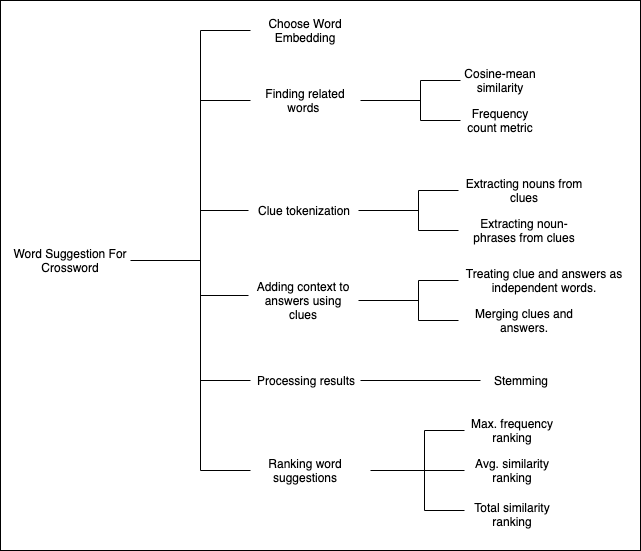
\includegraphics[width=300pt]{images/method_summary.png}
  \caption{Summary of techniques discussed for word suggestions for crosswords.}
  \label{fig:fig3.6.1}
\end{figure*}

\begin{figure*}
  \centering
  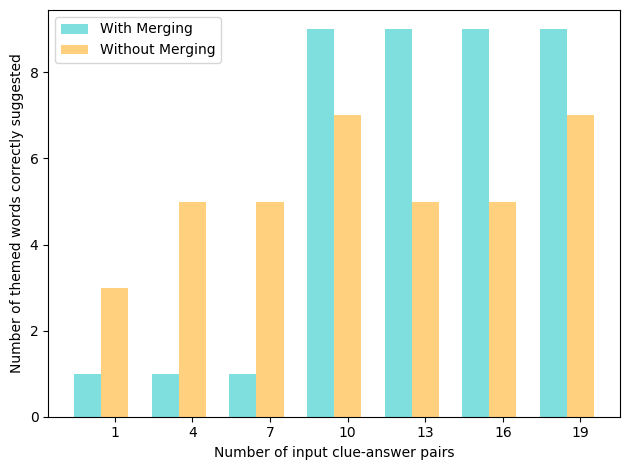
\includegraphics[height=150pt]{images/merging_vs_no_words_bar.png}
  \caption{Number of themed words correctly suggested out of top 10 words suggested based on input size.}
  \label{fig:fig3.6}
\end{figure*}

\begin{table}[h!]
  \begin{center}
    \begin{tabular}{c c c}
      \toprule
      \textbf{Max frequency ranking} & \textbf{Avg similarity ranking} & \textbf{Total similarity ranking}  \\ 
      \midrule
      Sabarmati Ashram & Bapu & Sabarmati Ashram \\
      Acharya Vinoba Bhave & Swami Vivekananda & Shivaji Maharaj\\
      Shivaji Maharaj & Pandit Nehru & satyagraha\\
      satyagraha & Shri Guruji & Acharya Vinoba Bhave\\
      Hind Swaraj & Hind Swaraj & Swami Vivekananda \\
	Sree Narayana Guru & Tagore & Bapu \\
       Ambedkar & Bhagat Singh & Ambedkar \\
      Pandit Nehru & Ambedkar & Hind Swaraj \\
      Bapu & Vinobha Bhave & Pandit Nehru \\
      Swami Vivekananda& Pandit Jawaharlal Nehru & Sree Narayana Guru \\
      \bottomrule
    \end{tabular}
    \caption{Top 10 word suggestions ranked for the Gandhi puzzle using different metrics.}
    \label{tab:table6}
  \end{center}
\end{table}

\section{Training on domain-specific corpus}
\label{sec:sec4}
For some problems, the topic may not be present (eg. a small city or village) or the topic not well represented (eg. Indian history may not be as well documented in news as by authors and biographers.) in the pretrained Google News model. Another major drawback of the Google News model is that the model is case-sensitive, as discussed in section \ref{sec:sec3.5}. Hence 'Gandhi' and 'gandhi' will have different vector representations. If we want to design puzzles which feel truly personal and special to the users, we cannot be limited by a pretrained model. Consider Dharwad, the home to the author's institute which is renowned for education, music and art. A simple query to the GoogleNews pretrained model to find the closest words to Dharwad include other well known cities. However, the model does not capture other aspects of Dharwad that are well known to the locals as Dharwad is not well-represented in the news. Figure \ref{fig:fig4.4.1} summarizes the strategies discussed for generating word embeddings from a domain-specific corpus.

\begin{figure*}
  \centering
  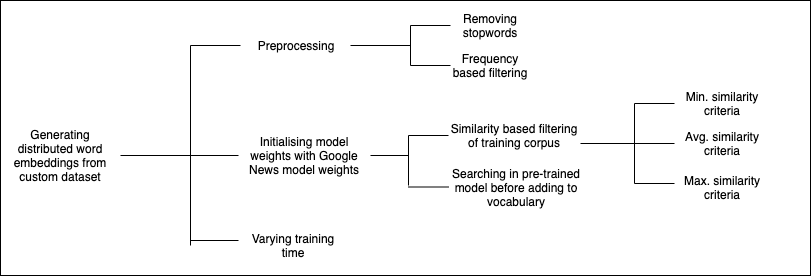
\includegraphics[width=\textwidth]{images/custom_training.png}
  \caption{Summary of techniques discussed for generating word embeddings from a domain-specific corpus.}
  \label{fig:fig4.4.1}
\end{figure*}

\subsection{Preprocessing}
Considering we have a set of documents on which we would like to train our model, the first step is to tokenize the document. Tokenization involves breaking a document into a list of sentences. Next, we clean up the document by removing all punctuations. Finally, we split each sentence into a list of words. Since we want our model to be case-insensitive, each word is converted to lower case. Table \ref{tab:table7} shows a small document before and after preprocessing.
\begin{table}[h!]
  \begin{center}
    \begin{tabular}{p{7cm} p{7cm}}
      \toprule
      \textbf{Before} & \textbf{After}  \\ 
      \midrule
      I would like to say to the diligent reader of my writings and to others who are
interested in them that I am not at all concerned with appearing to be
consistent. In my search after Truth I have discarded many ideas and learnt
many new things. & [['i', 'would', 'like', 'to', 'say', 'to', 'the', 'diligent', 'reader', 'of', 'my', 'writings', 'and', 'to', 'others', 'who', 'are', 'interested', 'in', 'them', 'that', 'i', 'am', 'not', 'at', 'all', 'concerned', 'with', 'appearing', 'to', 'be', 'consistent'], ['in', 'my', 'search', 'after', 'truth', 'i', 'have', 'discarded', 'many', 'ideas', 'and', 'learnt', 'many', 'new', 'things']] \\
    \bottomrule
    \end{tabular}
    \caption{Some lines of 'Hind Swaraj' by Gandhi, before and after preprocessing.}
    \label{tab:table7}
  \end{center}
\end{table}


\subsubsection{Stopwords}
Typically, documents contain many commonly used words such as “the”, “a”, “an”, “in” which are not useful. These words are known as stopwords and need to be removed before processing. Stop words take up valuable processing time, and dilute the context. Hence, we took a standard list of stop words (\textasciitilde1073 words) and filtered them out from the document. Table \ref{tab:table8} shows the document after preprocessing from \ref{tab:table7} before and after removing stop words. As we can observe, a lot of noise words have been removed.

\begin{table}[h!]
  \begin{center}
    \begin{tabular}{p{7cm} p{7cm}}
      \toprule
      \textbf{Before filtering stop words} & \textbf{After filtering stop words}  \\ 
      \hline
      	[['i', 'would', 'like', 'to', 'say', 'to', 'the', 'diligent', 'reader', 'of', 'my', 'writings', 'and', 'to', 'others', 'who', 'are', 'interested', 'in', 'them', 'that', 'i', 'am', 'not', 'at', 'all', 'concerned', 'with', 'appearing', 'to', 'be', 'consistent'], ['in', 'my', 'search', 'after', 'truth', 'i', 'have', 'discarded', 'many', 'ideas', 'and', 'learnt', 'many', 'new', 'things']] & [['reader', 'diligent', 'reader', 'writings', 'others', 'interested', 'concerned', 'appearing', 'consistent'], ['search', 'truth', 'discarded', 'ideas', 'learnt', 'things']] \\
      \bottomrule
    \end{tabular}
    \caption{Effect of removing stop words from the corpus. The lines are taken from 'Hind Swaraj' by Gandhi.}
    \label{tab:table8}
  \end{center}
\end{table}
\subsubsection{Frequency based filtering}
In addition to the standard stop words, we also considered removing the top K frequently occuring words from the corpus as they might not be useful. This could not be implemented as after removing the stopwords, the ten most frequently occuring words included 'Gandhi', 'India' and 'non-violence', among other important words.

\subsection{Result}
\label{sec:sec4.2}
 We trained the model using 14 books on Mahatma Gandhi, including his autobiographies and novels on his life. The total corpus contained 1,11,813 lines consisting of 8,04,432 words. The size of the vocabulary was 35,672. The training was done using both the Skip-gram model\footnote{Skip-gram model is designed to predict the context.} and the CBOW model\footnote{In CBOW, the model learns to predict the word by the context}. Table \ref{tab:table9} shows the words suggested by the model after training for the Gandhi puzzle. From the results, we observe that CBOW model performs better for this puzzle.

\begin{table}[h!]
  \begin{center}
    \begin{tabular}{c c}
      \toprule
      \textbf{Suggested Words (Skipgram Model)} & \textbf{Suggested Words (CBOW Model)}  \\ 
      \midrule
      \ul{lala} & \ul{vithalbhai} \\
      fazlul & \ul{rajagopalachari} \\
      hasan & \ul{besant}\\
      esq & monday\\
      vora & patna \\
      dutt & midnight \\
      carl & \ul{pyarelal} \\
      flew & \ul{devadas} \\
      deshpande & journey \\
      objecting & birthday \\
      \bottomrule
    \end{tabular}
    \caption{Top 10 word suggestions ranked for the Gandhi puzzle. The results in the first column are generated from a model trained on the Skip-Gram model. The results in the second column are generated from a model trained on the CBOW model. Both the models are trained on 14 books on Mahatma Gandhi. The themed words correctly suggested are highlighted in red.}
    \label{tab:table9}
  \end{center}
\end{table}  

\subsection{Initializing weights before training}
The good performance of the Google News dataset is due to the large text corpus it has been trained on, about 100 billion words. In reality, it is almost impossible to find this much amount of data for a specific topic to train the model. Hence, we proposed to exploit the Google News model information by initializing the weights of our model with the weights of the Google News model. The vocabulary was taken as a union of the vocabulary of the Google News model and the vocabulary of the domain-specific text corpus. In addition to this, we proposed two ideas to better preprocess the document:

\subsubsection{Similarity based filtering}
One intuitive idea is to filter the words which are semantically far from the input words. This makes sense as such words are not useful for our topic. Now, there are three possible ways to decide the criteria for filtering:
\begin{enumerate}
  \item Average Similarity Criteria: Filter if the average similarity of word from the input words is less than $ \epsilon$.
  \item Minimum Similarity Criteria: Filter if the minimum similarity of word from the input words is less than $\epsilon$.
  \item Maximum Similarity Criteria: Filter if the maximum similarity of word from the input words is less than $\epsilon$.
\end{enumerate}
Table \ref{tab:table10} shows the words suggested by the model after training for the Gandhi puzzle, with the training words filtered out according to different similarity criteria. From the results, we can observe that filtering significantly improves results. (Max. filtering may be same as no-filtering in this case as each word in the corpus may be having at least one word in the input list which is at least $\epsilon$-similar.)

\begin{table}[h!]
  \begin{center}
    \begin{tabular}{c c c}
      \toprule
      \textbf{Avg. Similarity} & \textbf{Min. Similarity} & \textbf{Max. Similarity} \\ 
      \midrule
      honour & \ul{Sabarmati Ashram} & spirit \\
      \ul{bhangi} & bhagavadgita & believe\\
      \ul{travancore} & \ul{tulsidas} & means\\
      gurudev & learnt & \ul{gokhale}\\
      never & \ul{comorin} & better \\
      \ul{transvaal} & neighbours & true \\
      labour & himalayas & possible\\
      country & parsi & world\\
      \ul{sanatanists} & \ul{coates} & nothing \\
      life & \ul{ishopanishad} & use \\
      \bottomrule
    \end{tabular}
    \caption{Top 10 word suggestions ranked for the Gandhi puzzle. The model has been initialized with the weights of the Google News model and training is done on 14 books on Mahatma Gandhi. Different filtering criteria have been used for preprocessing the document based on similarity (computed from Google News model) with input words. The themed words correctly suggested are highlighted in red.}
    \label{tab:table10}
  \end{center}
\end{table} 


\paragraph{Effect of varying $\epsilon$}{
In order to observe the dependence of the results on the similarity threshold ($\epsilon$), we varied $\epsilon$ and recorded the results for different values of $\epsilon$. Table \ref{tab:table11} shows the words suggested by the model after training for the Gandhi puzzle, with the training words filtered out according to different $\epsilon$ values. From the results, we can observe that the number of correct words do not vary significantly with different $\epsilon$ values (for the minimum-similarity criteria).}

\begin{table}[h!]
  \begin{center}
    \begin{tabular}{c c c}
      \toprule
      \textbf{$\epsilon=0.05$} & \textbf{$\epsilon=0.1$} & \textbf{$\epsilon=0.2$} \\ 
      \midrule
      \ul{Sabarmati Ashram} & \ul{Sabarmati Ashram} & \ul{Sabarmati Ashram} \\
      neighbour & bhagavadgita & zoroastrianism\\
      zoroastrianism & \ul{tulsidas} & selfcontrol\\
      bhagavadgita & learnt & \ul{varnashram}\\
      \ul{moonje} & \ul{comorin} & \ul{satyagrahi} \\
      \ul{tulsidas} & neighbours & neighbour \\
      \ul{tolstoy} & himalayas & \ul{tulsidas}\\
      devanagari & parsi & \ul{gandhijinnah}\\
      \ul{karamchand} & \ul{coates} & godfearing \\
      huq & \ul{ishopanishad} & bhagavadgita \\
      \bottomrule
    \end{tabular}
    \caption{Top 10 word suggestions ranked for the Gandhi puzzle. The model has been initialized with the weights of the Google News model and training is done on 14 books on Mahatma Gandhi. Different values of $\epsilon$ have been used for preprocessing the document based on minimum similarity criteria (computed from Google News model) with input words. The themed words correctly suggested are highlighted in red.}
    \label{tab:table11}
  \end{center}
\end{table} 


\subsubsection{Searching in model before adding to vocabulary}
Since not all words in the training corpus would necessarily be in the Google News model vocabulary, we simply retain such words. Also, in order to not have two vector representations for the same word, we first query the Google News model to find if any other case (uppercase, titlecase) of the word is already present in the model vocabulary. If present, we replace the word in our corpus with the case followed by the Google News word.

\subsection{Effect of training time}
We decided to increase the training time as increasing the number of epochs usually benefits the quality of the word representations. Table \ref{tab:table12} shows the words suggested by the model after training for the Gandhi puzzle, with increasing training time. From the results, it cannot be said if training longer definitely improves results.

\begin{table}[h!]
  \begin{center}
    \begin{tabular}{c c c c}
      \toprule
      \textbf{$epochs=5$} & \textbf{$epochs=15$} & \textbf{$epochs=25$} & \textbf{$epochs=35$}  \\ 
      \midrule
      \ul{Sabarmati Ashram} & know & true & \ul{yeravda} \\
      zoroastrianism & use & centre & \ul{mahatmaji}\\
      selfcontrol & labour & \ul{sevagram} & \ul{tolstoy}\\
      \ul{varnashram} & truth & \ul{santiniketan} & gita\\
      \ul{satyagrahi} & \ul{tagore} & know & kshitimohanbabu\\
      neighbour & never & \ul{antiuntouchability} & lessmore\\
      \ul{tulsidas} & country & today & oversight…\\
      \ul{gandhijinnah} & \ul{yeravda} & \ul{rajkot} & orlov\\
      godfearing & \ul{gandhiji} & \ul{hindumuslim} & iare\\
      bhagavadgita & long & \ul{rolland} & \ul{segaon} \\
      \bottomrule
    \end{tabular}
    \caption{Top 10 word suggestions ranked for the Gandhi puzzle. The model has been initialized with the weights of the Google News model and training is done on 14 books on Mahatma Gandhi, with increasing training time. The themed words correctly suggested are highlighted in red.}
    \label{tab:table12}
  \end{center}
\end{table} 

\section{Deriving relations between clues and answers}
\label{sec:sec5}
We wanted to derive relations between clues and answers. For example, if the user suggests 'Paris' as answer and '$\rule{1cm}{0.15mm}$ : capital of France' as the clue, we wanted to see if we could suggest 'New Delhi' as answer and '$\rule{1cm}{0.15mm}$ : capital of India' as the clue. An analogy question is a question that asks one to find the relationship between words. For instance, the answer to the question: man is to woman, what king is to $\rule{1cm}{0.15mm}$ is “queen” since we have to use the relationship in the first part of the question to fill in the blank. Now, it has been shown that given words $a$, $b$ and $c$, using vector representations produced by Word2Vec we can find $d$ such that it satisfies $a:b::c:d$ \cite{cite16}. $d$ is such that vec(d) is closest to vec(c) + vec(b) - vec(a) according to cosine distance (we discard the input words from the search).

One possible way of attempting this is as follows: we take the answer word $a$ and for each word $c_i$ in the clue, we do the following. Let $N(a)$ be the $m$ nearest neighbours of a and $N(c_i)$ be the $n$ nearest neighbours of $c_i$. Now for every pair $(x, y)$ in $N(a) \times N(c_i)$, check if $y$ satisfies equation \ref{eq:eq1}. If $y$ satisfies the equation, output a new clue-answer pair where $a_{new}$ = $x$ and $c_{new} = c.replace(c_i, y)$. 

\begin{equation}
\label{eq:eq1}
vec(y) = \argmin_{vec(z)}{D(vec(z), vec(c_i) - vec(a) + vec(x))}
\end{equation}
where $D(a,b)$ is the cosine distance between $a$ and $b$.


\begin{figure*}
  \centering
  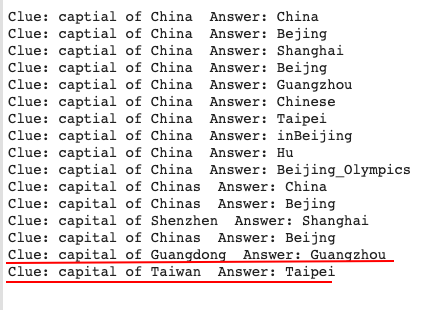
\includegraphics[height=200pt]{images/analogies.png}
  \caption{Attempt to derive similar clues and answer pairs from the clue "$\rule{1cm}{0.15mm}$ : capital of China" and answer "Beijing". Out of the 16 suggestions, only two are correct (highlighted in red).}
  \label{fig:fig4}
\end{figure*}

Figure \ref{fig:fig4} shows the result of applying our naive algorithm to the clue "$\rule{1cm}{0.15mm}$ : capital of China" and answer "Beijing". As we can observe, only two correct capital:country/province relation was captured. It is interesting to note that Word2Vec captures many false relations too. If the given word $c$ is not of the same category as $a$, it will find a $d$ it thinks is related to $c$ in the same manner as $a$ is related to $b$. Thus, to obtain the correct relation, one must ensure that $c$ is of the same type as $a$.

\section{System Development}
\label{sec:sec6}
In this section, we cover the details of our system implementation that led to the final product prototype. There were mainly two requirements for the system: (1) API-based recommendations which can be integrated with Amuse Lab's products such as Crossword, Wordsearch etc. (2) Web-based GUI for experiments and debugging. In Figure \ref{fig:fig3} we show an example of our word recommender, where 'sandesh', 'modak' and 'halwa' are suggested after some Indian sweets themed clues and words are given as input.

\begin{figure*}
  \centering
  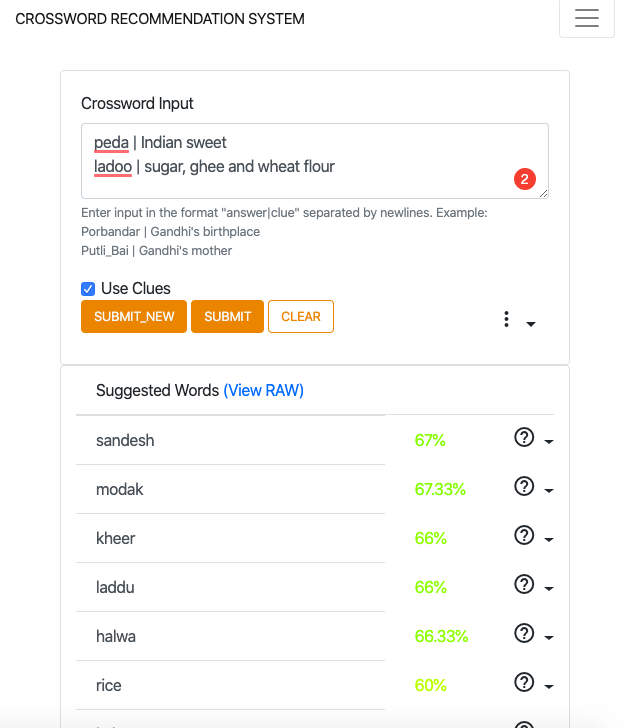
\includegraphics[height=250pt]{images/sweet_example.png}
  \caption{Word recommendation product for Amuse Labs crosswords.}
  \label{fig:fig3}
\end{figure*}

\subsection{API}
A python-based server listens for GET requests at /similar-words. The request accepts two query parameters: words and clues, which are list of strings. The response consists of four fields: (1) \verb|suggested_words|: the words suggested for the crossword, (2) \verb|words_not_in_vocab|: to prompt user that an input word is not present in the model's vocabulary, (3) \verb|words_map|: to capture the input words which have generated a result word, along with their cosine similarity (for debugging and understanding the results), and (4) \verb|clue_nouns|: to capture the noun words extracted from the clues (for debugging). Figure \ref{fig:fig5} shows a sample API response for the query \verb|similar-words/?words=peda&clues=Indian%20sweet&words=kheer&clues=sweet%20and%20milk|.
\begin{figure*}
  \centering
  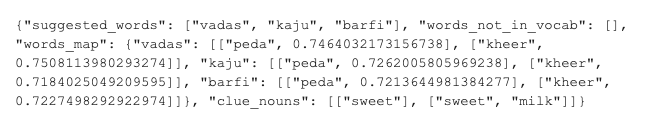
\includegraphics[width=\textwidth]{images/api_demo.png}
  \caption{Sample API response for two clues and answers. The results have been truncated for ease of understanding.}
  \label{fig:fig5}
\end{figure*}

\subsection{GUI}
For the Graphical User Interface, we created an interactive web application which renders the API response in Javascript and HTML. The requests are made asynchronously using AJAX for seamless use, and are made either at the press of the submit button or pressing of ENTER key (after a clue-answer pair has been input). It supports adding words from the suggestions to the input (positive feedback) with a click, displays the input words responsible for a particular result word, displays color-coded score of each word (computed from input word cosine-similarities), supports viewing the nouns extracted from the clues and also allows to disable clues.
\subsection{Timing issues}
Using the system realtime, we found that the response time grows proportionally with the size of the input. For example, for an input of 19 clue-answer pairs, it takes \textasciitilde 17s for the response to return. Since, this is meant to be an interactive system, we cannot accept this much delay. On a careful analysis, we found that the most expensive operation of the algorithm is \verb|model.most_similar()| which finds the $k$ closest words for the given word as it searches in the entire model vector space. We proposed the idea to cache the top $k$ similar words for each input word in a per-user session. This is because one word may be common across different clues, and more importantly, typically a user will enter the input line-by-line. We do not want to reprocess the previous input. Hence, after implementing caching, the average response time became $< 1 s$.

\section{Discussion}
\label{sec:sec7}
We would like to highlight few limitations of our work. First, the quality of suggestions degrades as the scope of the theme becomes more broad. For example, in the example we considered, the theme was highly specific due to which we were able to get very good results. If the theme is more general such as sports, the results may or may not be as good depending on the input. Secondly, the embeddings generated from a custom dataset cannot replace the embeddings from Google News as they have been trained on a significantly larger dataset and more sophisticated processors. The results can, in most cases, only supplement the results from a pretrained model. 
Our work to derive relations between clues and answers was preliminary and needs to be extended for practical use. All evaluations have been done qualitatively and the techniques have been developed using several heuristic based approaches.\\ In spite of these, we have considered many real-life themed puzzles and observed that our algorithm works well in most cases, and can help in a richer fill. We are able to fine-tune and apply the idea of word-vector representation to our particular use case of crosswords.  This, in itself, is quite significant as we are able to introduce state-of-the-art machine learning techniques to crosswords.


\section{Conclusions and Future Work}
\label{sec:sec8}
In this report we proposed a novel technique for suggesting words for crosswords that leverages understanding of word semantics using high-dimensional word vectors. We showed that our algorithm works well to extract
a theme across a given set of clues and answers, and is able to give themed suggestions. Further, we provided serveral strategies for using clues, generating suggestions, ranking the words and generating embeddings from a domain-specific corpus. Since the word embeddings can be generated over any text corpus in an unsupervised fashion, our technique will work well for highly specialized domain crosswords too. We also presented the details of a system developed which is able to give near real-time word suggestions to the users.
\\ The next step could be to extend our algorithm to use the topic modeling techniques (LDA2Vec)\cite{cite25} and document embeddings (Doc2Vec)\cite{cite24}. We can utilize user feedback to further improve the performance of our word recommendation system. We can also have a rule based system which captures the most common categories of clue-answer pairs for automatic clue suggestions.


\section{Acknowledgements}
The author would like to thank Prof. Prabuchandran KJ and Prof. Sudheendra Hangal for guiding this project and for giving their invaluable time and input. The author would also like to thank Dept. of Computer Science and Engineering, IIT Dharwad, for providing the opportunity to work on this project.
%----------------------------------------------------------------------------------------
%	REFERENCE LIST
%----------------------------------------------------------------------------------------

\begin{thebibliography}{99} % Bibliography - this is intentionally simple in this template
\bibitem [1]{cite1}
Edward K. Crossman \& Sharyn M. Crossman (1983)
\newblock The Crossword Puzzle as a Teaching Tool, 
\newblock Teaching of Psychology, 10:2, 98-99, DOI: {\em \href{https://doi.org/10.1207/s15328023top1002_10}{10.1207/s15328023top1002\_10}}.

\bibitem [2]{cite2}
Childers, Cheryl D.
\newblock “Using Crossword Puzzles as an Aid to Studying Sociological Concepts.” 
\newblock Teaching Sociology, vol. 24, no. 2, 1996, pp. 231–235. JSTOR, {\em \href{www.jstor.org/stable/1318816}{www.jstor.org/stable/1318816}}.

\bibitem [3]{cite3}
Anurag  Saxena  and  Raenelle  Nesbitt  and  Punam  Pahwa  and  Sheryl  Mills.
\newblock Crossword Puzzles: Active Learning in Undergraduate Pathology and Medical Education, 
\newblock Archives of Pathology \& Laboratory Medicine, vol. 133, no. 9, 2009, pp. 1457-1462, DOI: {\em \href{www.archivesofpathology.org/doi/pdf/10.1043/1543-2165-133.9.1457}{10.1043/1543-2165-133.9.1457}}.

\bibitem [4]{cite4}
M. L. Ginsberg et al.
\newblock Search Lessons Learned From Crossword Puzzles.
\newblock AAAI'90 Proceedings of the eighth National conference on Artificial intelligence - Volume 1
Pages 210-215. Available {\em \href{https://pdfs.semanticscholar.org/1de1/b304d476488a4de29bedadd40364904c7637.pdf}{here}}

\bibitem [5]{cite5}
L. J. Mazlack.
\newblock Computer Construction of Crossword Puzzles Using Precedence Relationships 
\newblock  Articial Intelligence 7, pp 1\{19, 1976. DOI: {\em \href{https://doi.org/10.1016/0004-3702(76)90019-9}{10.1016/0004-3702(76)90019-9}}.

\bibitem [6]{cite6}
M. L. Ginsberg (2011).
\newblock Dr.Fill: Crosswords and an Implemented Solver for Singly Weighted CSPs
\newblock  Jair.org. Retrieved 2012-03-12. {\em \href{http://www.jair.org/papers/paper3437.html}{http://www.jair.org/papers/paper3437.html}}.

\bibitem [7]{cite7}
L. Rigutini, M. Diligenti, M. Maggini, and M. Gori,
\newblock “Automatic generation of crossword puzzles,”
\newblock  International Journal on Artificial Intelligence Tools, vol. 21, no. 03, 2012. [Online]. Available: {\em \href{https://doi.org/10.1142/S0218213012500145}{https://doi.org/10.1142/S0218213012500145}}.

\bibitem [8]{cite8}
Aherne, A. \& C. Vogel (2006). 
\newblock Wordnet enhanced automatic crossword generation.
\newblock  In P. Sojka, K.-S. Choi, C. Fellbaum, \& P. Vossen (Eds.), Proceedings of the Third International Wordnet Conference, pp. 139 – 145.  Available {\em \href{https://www.scss.tcd.ie/disciplines/intelligent_systems/clg/clg_web/ahernevogel06.pdf}{here}}.

\bibitem [9]{cite9}
Y. Bengio, R. Ducharme, P. Vincent, and C. Janvin. (2003). 
\newblock  A neural probabilistic language model.
\newblock  J. Mach. Learn. Res., 3:1137–1155

\bibitem [10]{cite10}
R. Collobert and J. Weston. (2008). 
\newblock  A unified architecture for natural language processing: Deep neural networks with multitask learning.
\newblock  In Proceedings of the 25th International Conference on Machine Learning, ICML ’08, pages 160–167, New York, NY, USA, 2008. ACM.

\bibitem [11]{cite11}
R. Collobert, J. Weston, L. Bottou, M. Karlen, K. Kavukcuoglu, and P. Kuksa. (2011). 
\newblock  Natural language processing (almost) from scratch.
\newblock  J. Mach. Learn. Res., 12:2493–2537, Nov. 2011.

\bibitem [12]{cite12}
A. Mnih and G. E. Hinton. (2009). 
\newblock  A scalable hierarchical distributed language model.
\newblock  In Advances in neural information processing systems, pages 1081–1088, 2009.

\bibitem [13]{cite13}
 J. Turian, L. Ratinov, and Y. Bengio. (2010). 
\newblock  Word representations: a simple and general method for semi-supervised learning.
\newblock In Proceedings of the 48th annual meeting of the association for computational linguistics, pages 384–394. Association for Computational Linguistics, 2010.

\bibitem [14]{cite14}
 E. H. Huang, R. Socher, C. D. Manning, and A. Y. Ng. (2012). 
\newblock  Improving word representations via global context and multiple word prototypes.
\newblock In Proceedings of the 50th Annual Meeting of the Association for Computational Linguistics: Long Papers - Volume 1, ACL ’12, pages 873–882, Stroudsburg, PA, USA, 2012. Association for Computational Linguistics

\bibitem [15]{cite15}
  T. Mikolov, K. Chen, G. Corrado, and J. Dean (2013). 
\newblock Efficient estimation of word representations in vector space.
\newblock CoRR, abs/1301.3781, 2013.

\bibitem [16]{cite16}
 T. Mikolov, I. Sutskever, K. Chen, G. S. Corrado, and J. Dean (2013). 
\newblock Distributed representations of words and phrases and their compositionality.
\newblock In C. Burges, L. Bottou, M. Welling, Z. Ghahramani, and K. Weinberger, editors, Advances in Neural Information Processing Systems 26, pages 3111–3119. Curran Associates, Inc., 2013.

\bibitem [17]{cite17}
 T. Mikolov, W.-T. Yih, and G. Zweig (2013). 
\newblock Linguistic regularities in continuous space word representations.
\newblock In HLT-NAACL, pages 746–751, 2013.

\bibitem [18]{cite18}
J. Pennington, R. Socher, and C. D. Manning (2014). 
\newblock  Glove: Global vectors for word representation.
\newblock In EMNLP, volume 14, pages 1532–1543, 2014.

\bibitem [19]{cite19}
R. Socher, E. H. Huang, J. Pennin, C. D. Manning, and A. Y. Ng (2011). 
\newblock  Dynamic pooling and unfolding recursive auto-encoders for paraphrase detection.
\newblock In Advances in Neural Information Processing Systems, pages 801–809, 2011.

\bibitem [20]{cite20}
R. Socher, C. C. Lin, C. Manning, and A. Y. Ng (2011). 
\newblock  Parsing natural scenes and natural language with recursive neural networks.
\newblock In Proceedings of the 28th international conference on machine learning (ICML-11), pages 129–136, 2011.

\bibitem [21]{cite21}
A. Kumar, O. Irsoy, J. Su, J. Bradbury, R. English, B. Pierce, P. Ondruska, I. Gulrajani, and R. Socher (2015). 
\newblock  Ask me anything: Dynamic memory networks for natural language processing.
\newblock arXiv preprint arXiv:1506.07285, 2015.

\bibitem [22]{cite22}
J. Weston, A. Bordes, S. Chopra, and T. Mikolov (2015). 
\newblock  Towards ai-complete question answering: A set of prerequisite toy tasks.
\newblock arXiv preprint arXiv:1502.05698, 2015.

\bibitem [23]{cite23}
M. Grbovic, V. Radosavljevic, N. Djuric, N. Bhamidipati, J. Savla, V. Bhagwan, and D. Sharp (2015). 
\newblock  E-commerce in your inbox: Product recommendations at scale.
\newblock In Proceedings of the 21th ACM SIGKDD International Conference on Knowledge Discovery and Data Mining, KDD ’15, pages 1809–1818, New York, NY, USA, 2015. ACM.

\bibitem [24]{cite24}
Le, T. Mikolov. (2014). 
\newblock  Distributed Represenations of Sentences and Documents.
\newblock In Proceedings of ICML 2014.

\bibitem [25]{cite25}
Moody, Christopher E. (2016). 
\newblock  Mixing dirichlet topic models and word embeddings to make lda2vec.
\newblock arXiv preprint arXiv:1605.02019, 2016.

\bibitem [26]{cite26}
Tan J. (2017). 
\newblock  24 Years of NYT Crossword Answers.
\newblock {\em https://jtanwk.github.io/nytcrossword/}.

\end{thebibliography}
%----------------------------------------------------------------------------------------

\end{document}
